\chapter{Evaluation}
\label{chap:num_6}

This chapter briefly describes and evaluates the results, recognition, and notable achievements obtained after evaluating final \lpas{} solution inside the production instance of \lpa{} platform \footnote{\url{https://applications.linkedpipes.com}}.

\section{Benefits of \solid{}}

Usage of \solid{} technology significantly enhanced the initial functionality of \lpa{}, allowing to utilize the full benefits of Semantic Web and Linked Data management. The section describes the individual advantages and their influence on the improvement of \lpa{} platform.

\subsection{ACL managed applications}

Access Control Management is one of the core features provided by \solid{}. The implementation and integration of \textit{AccessControManager} abstraction from \lpas{} package, ability for \lpa{} developers to easily create, and edit the ACL files. From the perspective of \lpa{} platform users, this provided the ability to have full control and management over the data created by the \lpa{} but stored in \lpas{} package. 

\subsection{Everything is an RDF resource}

Storing \lpa{} applications in \solid{} means storing their configuration files expressed in TTL RDF format. Therefore, adding more value to the date as it can be queried, filtered, or transformed in any way possible using SPARQL querying language. Consider a use case where an experienced data journalist and developer who created and owns a set of multiple visualizers displaying markers on a map, he recently discovered a new dataset that consists of smaller datasets for applications he created previously. He can use SPARQL to analyze his configurations stored in his \solid{} POD and create a new configuration by aggregating the filters from smaller application configurations and \lpa{} platform will attempt to re-create the application for a new configuration.
Storing data as RDF also provides possibilities for future enhancements of \lpas{}. For instance, consider a case when several \lpa{} applications are embedded in a service similar to Wikipedia. One could easily create a SPARQL query to extract URIs to those visualizations and query any of the components of that configuration. 

\subsection{Provider agnostic storage}

By design, \solid{} servers are decentralized, a single \solid{} POD can host multiple \solid{} POD, and user own the data inside each of the PODs. When an \lpa{} platform users creates his first WebID and a \solid{} POD, all of \lpa{} configurations are created inside the \solid{} POD in authenticated \solid{} server. However, it is not bound to any specific implementation of \solid{} servers, it is completely agnostic and supports any implementation of a server that complies to \solid{} specification. In addition to that, user has an ability to use the \textit{Storage Control Panel} to move the created configurations within their PODs. The \solid{} POD webpage also allows users to move any data between different instances of \solid{} servers.

\section{Results and achievements}

The sections provide a brief overview of notable achievements and recognitions of \lpa{} platform that was directly and indirectly influenced by usage of \solid{} technology. 

\subsection{Recognition on official \solid{} website}
\label{sssec:recogniition_on_solid}

In July 2019, after the first production release of \lpa{} platform with a partial implementation of \lpas{}, the project was approved and added into the official list of \solid{} applications on the repository of \solid{} organization in GitHub. The screenshot of \autoref{fig:lpa_listing_on_solid} demonstrates the listing of the project on the official website.

\begin{figure}[h]
\centering
\fcolorbox{black}{white}{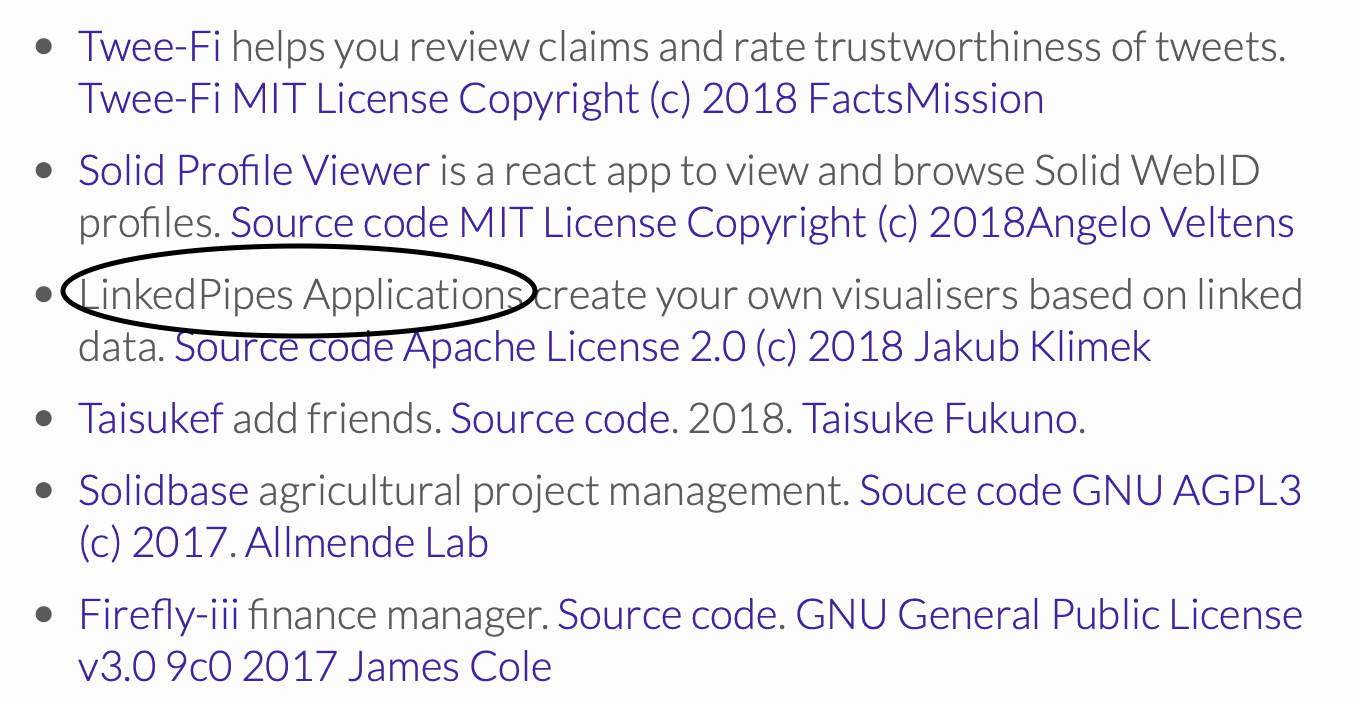
\includegraphics[width=0.7\linewidth]{lpa_listing_on_solid.png}}
\caption{Listing of \lpa{} platform on official \solid{} project website.}
\label{fig:lpa_listing_on_solid}
\end{figure}

\subsection{Comments from Sir Tim Berners-Lee}
\label{sssec:comments_from_tim}

During the whole development lifecycle of the \lpas{} project, active communication with the community helped to clarify many intricated nuances in the rapidly changing development ecosystem of \solid{} project. The creator of the \solid{} project is an active participant on \textit{Gitter} \footnote{\url{https://gitter.im}} channels related to the project. During the implementation of \textit{FileManager} abstraction, multiple questions asked on \solid{} channels on Gitter were answered by Sir Tim Berners-Lee, providing useful insights and motivation to contribute into the development of \solid{} as a web standard for decoupling and decentralizing the web. One of several interactions is demonstrated on a screenshot of a conversation of \autoref{fig:comments_from_tim_bl}.

\begin{figure}[h]
\centering
\fcolorbox{black}{white}{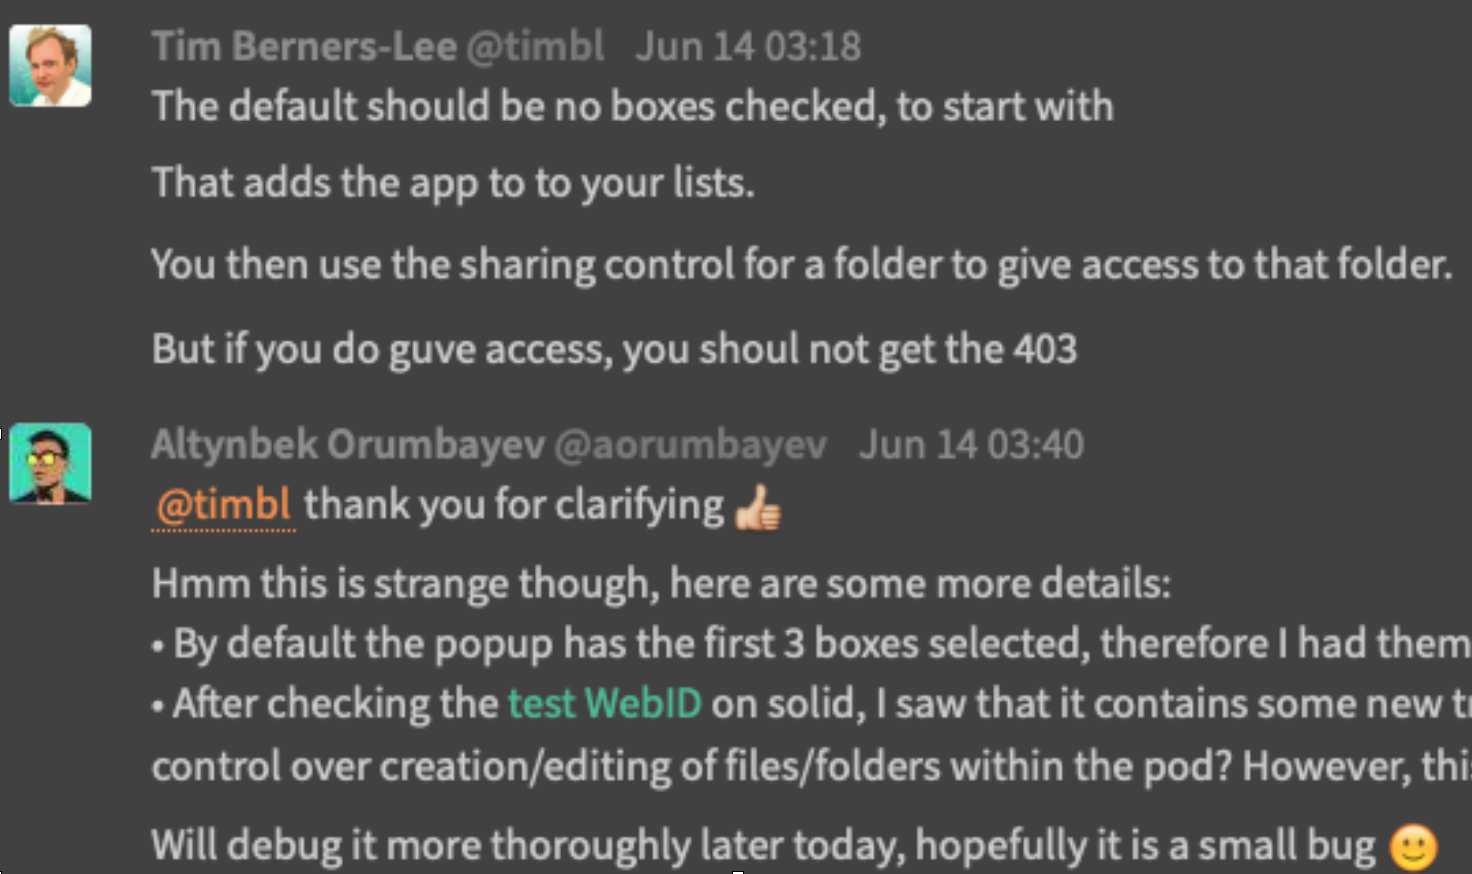
\includegraphics[width=0.7\linewidth]{comments_from_tim_bl.png}}
\caption{One of multiple interactions with creator of \solid{} on \solid{} community chat.}
\label{fig:comments_from_tim_bl}
\end{figure}

\subsection{User traction on \lpa{} platform}
\label{sssec:user_traction_of_platform}

Evaluation of final release of \lpa{} platform with finalized \lpas{} solution received a feedback from multiple \solid{} community members. Additionally one of the members of \gls{BARTOC} organization evaluated the application, provided a positive feedback and published an application stored in \solid{} using \lpas{} on official website of organization \footnote{\url{https://new.bartoc.org/node/332}}. It is important to note that the evaluators from BARTOC were using a beta staging version of the \lpa{} platform. Therefore the live instance available on their website may not be available due to database updates after the final release of the platform in July 2019.

\begin{figure}[hbt]
\minipage{0.4\textwidth}
  \fcolorbox{black}{white}{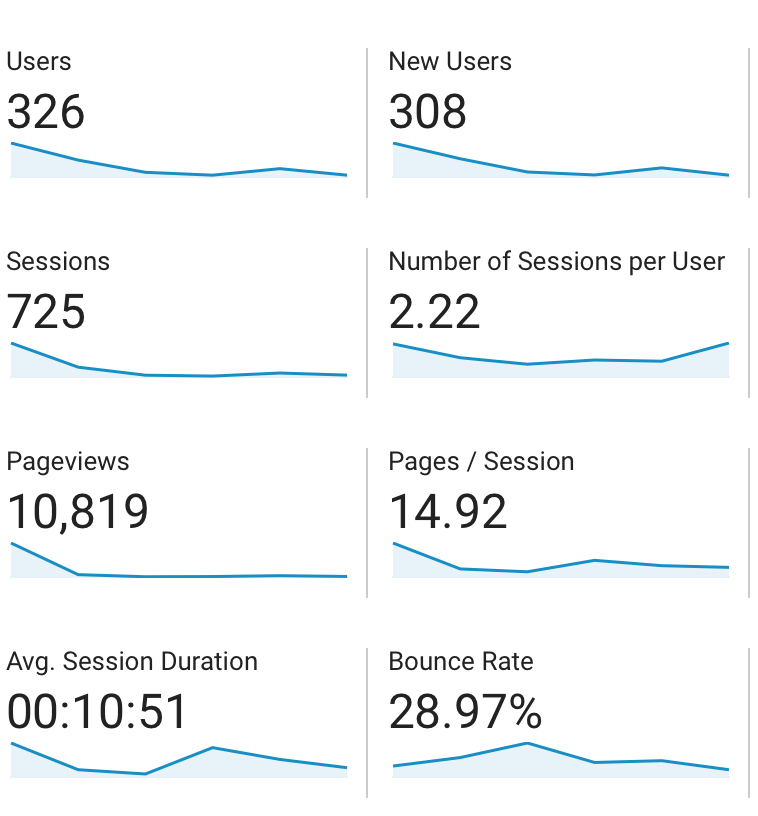
\includegraphics[width=0.8\linewidth]{google_analytics_users.png}}
  \caption{Google Analytics traction of users of test \lpa{} platform instance over a period of six months.}
  \label{fig:google_analytics_users}
\endminipage\hfill
\minipage{0.6\textwidth}
  \fcolorbox{black}{white}{
\includegraphics[width=0.8\linewidth]{community_post_users.png}}
  \caption{Feedback, views and comments on for \lpa{} launch on official \solid{} community forum.}
  \label{fig:community_post_users}
\endminipage\hfill
\end{figure}

Additionally, screenshots on \autoref{fig:google_analytics_users} and \autoref{fig:community_post_users} demonstrate the traction of \solid{} community users. Release of the \lpa{} platform with \lpas{} storage was posted on official \solid{} community forum, where a notable positive commentary was left by one of the founders of \textit{Virtuoso Universal Server} Kingsley Uyi Idehen \footnote{\url{http://dbpedia.org/page/Kingsley_Uyi_Idehen}}. Over the period of six month starting July and ending on December 2019, over 300 users interacted with test instance of \lpa{} as demonstrated on \autoref{fig:google_analytics_users}.